\documentclass{exam}
\usepackage[utf8]{inputenc}
\usepackage{upgreek}
\usepackage[margin=1in]{geometry}
\usepackage{amsmath,amssymb}
\usepackage{multicol}
\usepackage{stmaryrd}
\usepackage{graphicx}
\usepackage{caption}
\usepackage{tikz}
\usepackage{dsfont}
\usepackage{enumitem}
\usepackage{hyperref}
\usetikzlibrary{matrix}
\newcommand\tab[1][1cm]{\hspace*{#1}}
\pagestyle{head}
\firstpageheader{}{}{}
\runningheader{\examnum}{\class}{\name}
\runningheadrule
\newcommand{\class}{Fundamentos de bases de datos}
\newcommand{\term}{Facultad de Ciencias UNAM}
\newcommand{\examnum}{Tarea 03}
\newcommand{\examdate}{22/04/2022}
\newcommand{\name}{Jurassic Team}
\begin{document}

\noindent
\begin{tabular*}{\textwidth}{l @{\extracolsep{\fill}} r @{\extracolsep{6pt}} l}
\textbf{\class} & \textbf{\term}\\
\textbf{\examnum} & \textbf{\name}\\
\textbf{\examdate}
\end{tabular*}\\
\rule[2ex]{\textwidth}{2pt}

\section*{Preguntas}
%AQUI VAN LAS PREGUNTAS
\begin{questions}
	\question \textbf{Preguntas de repaso}
	
	\begin{enumerate}[label=\roman*.]
		\item ¿Qué es una relación y qué características tiene?
		
		\item ¿Qué es una llave primaria?, ¿qué es una llave candidata?, ¿qué es una llave natural?
		
		\item ¿Qué restricciones impone una llave primaria y una llave foránea al modelo de datos relacional?
		
		\item Investiga que cuáles son las Reglas de Codd y explica con tus propias palabras cinco reglas que consideres
interesantes. Indica por qué consideras que son importantes.
	\end{enumerate}
	
	\question \textbf{Modelo relacional}
	\begin{enumerate}[label=\alph*.]
		\item Traduce el siguiente modelo Entidad – Relación a su correspondiente Modelo Relacional:
		\begin{figure}[h!]
			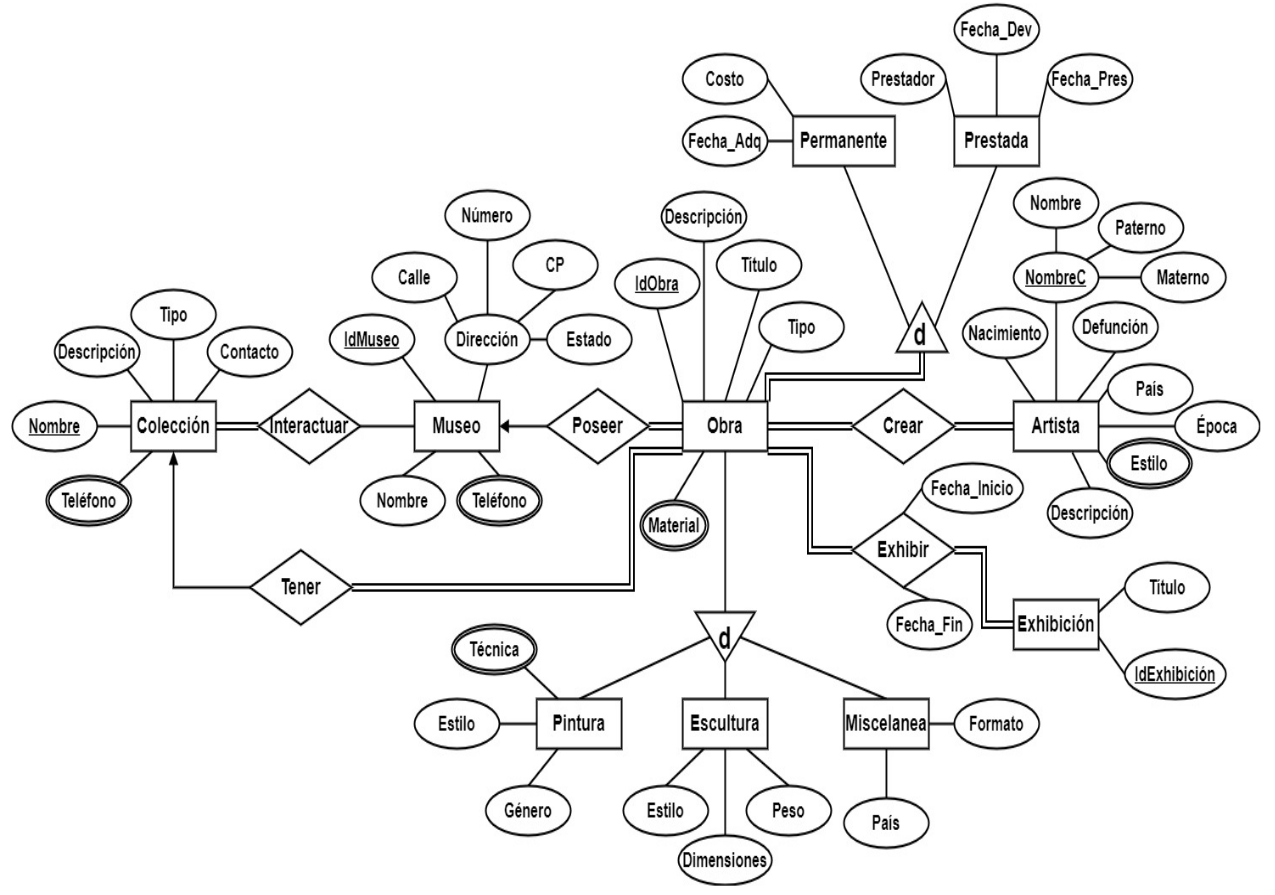
\includegraphics[width=18cm]{pregunta_2_a.png}
		\centering
		\end{figure}
	\end{enumerate}
	\question \textbf{Modelo relacional e inserción de tuplas}
	
	Considera el siguiente Modelo E/R:
	\begin{figure}[h!]
			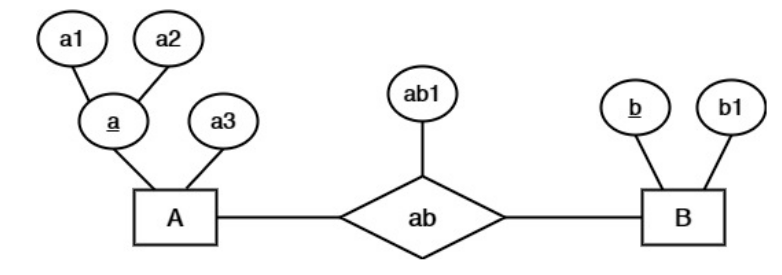
\includegraphics[width=10cm]{pregunta_3.png}
		\centering
		\end{figure}
		\begin{enumerate}[label=\alph*.]
			\item Completa la tabla que se presenta a continuación, convirtiendo el Modelo E-R en un Modelo Relacional, para todas
las opciones de cardinalidad (considera en todos los casos, participación parcial). Indica las relaciones resultantes,
su llave primaria y la integridad referencial. Utiliza el formato Tabla (llave, atr1, atr2,…,atrN).
			\begin{figure}[h!]
			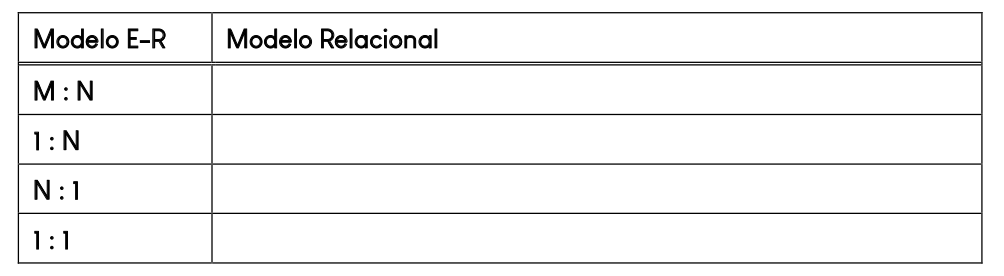
\includegraphics[width=13cm]{pregunta_3_a.png}
		    \centering
		    \end{figure}
			\item Del inciso a) toma el MR que obtuviste para la cardinalidad M:N. Asume que los atributos a1, b y ab1 son de tipo
entero, mientras que a2, a3 y b1 son de tipo cadena. Supón que la relación A tiene 4 tuplas con los siguientes valores
(2,’ww’,’a’), (4,’xx’,’b’), (6,’yy’,’c’), (8,’zz’,’d’) y la relación B tiene 5 tuplas identificadas por
los valores 17, 27, 37, 47, 57. Los incisos que se presentan a continuación, representan un conjunto de tuplas
a insertar (en ese orden) en la relación AB, indica cuál conjunto se puede insertar completamente en dicha relación.
Justifica tu respuesta en cada caso.
\begin{enumerate}[label=\roman*.]
				\item (8,’zz’,17,5); (6,’yy’,57,10); (4,’xx’,27,15); (2,’ww’,37,20); (4,’xx’,27,15)
				\item (17,’zz’,2,’m’); (27,’yy’,4,’n’); (37,’xx’,6,’o’); (47,’ww’,8,’p’); (57,’zz’,4,’q’)
				\item (2,’a’,17,23); (4,’b’,27,24); (6,’c’,37,25); (8,’d’,47,26); (2,’a’,57,27)
				\item (2,’ww’,57,’a’); (4,’xx’,37,’a’); (6,’yy’,17,’a’); (8,’zz’,17,’a’); (10,’xx’,27,’a’)
\end{enumerate}
           \item Del inciso a) toma como base el MR que obtuviste para la cardinalidad 1:N. Los incisos que se presentan a
continuación representan un conjunto de tuplas a insertar (en ese orden) en la relación B, indica cuál conjunto se
puede insertar completamente en dicha relación. Justifica tu respuesta en cada caso.  
\begin{enumerate}[label=\roman*.]
				\item (2,’f’,57,’zz’); (4,’g’,47,’yy’); (6,’h’,37,’xx’); (8,’i’,27,’ww’); (2,’j’,17,’yy’)
				\item (17,’ww’); (27,’xx’); (37,’yy’); (47,’zz’); (57,’zz’); (17,’xx’); (27,’yy’)
				\item (57,’f’,8,’zz’); (47,’g’,6,’yy’); (37,’h’,4,’xx’); (27,’i’,2,’ww’); (17,’j’,6,’yy’)
				\item (57,’f’,8,’a’); (47,’g’,6,’b’); (37,’h’,4,’c’); (27,’i’,2,’d’); (17,’j’,6,’c’)
\end{enumerate}
			\item Considera el mismo escenario del inciso b para las relaciones A y B. Toma como base el Modelo Relacional que
obtuviste para la cardinalidad 1:1. Supón que tu modelo tiene participación total del lado de la relación A. Propón
un conjunto de 4 tuplas que se pueda insertar en A y un conjunto que no se pueda insertar (también de 4 tuplas).
Justifica tu respuesta en cada caso.
			\end{enumerate}
	
	\question \textbf{Modelo relaciones y restricciones de integridad}
	
	A continuación, se encuentra el Modelo Relacional de un departamento de recursos humanos que controla varias
empresas. En este esquema, supón que desde es inclusivo, mientras que hasta es exclusivo, definiendo el período
[desde,hasta). Indica si las siguientes afirmaciones se cumplen o no. Justifica tu respuesta (solo considera las
restricciones que se indican en el esquema):
	
	\begin{figure}[h!]
		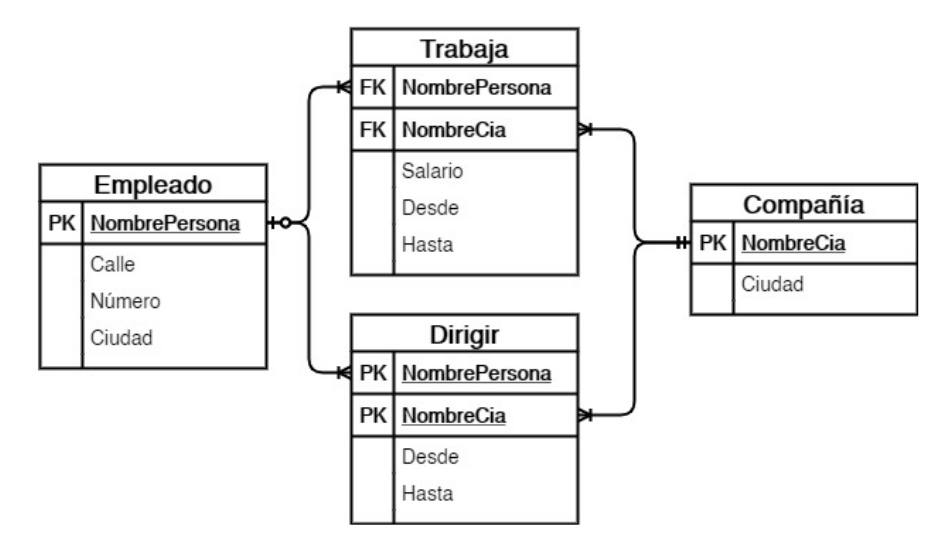
\includegraphics[width=15cm]{pregunta_4.png}
		\centering
	\end{figure}
	
	\begin{enumerate}[label=\alph*.]
		\item Dos o más compañías con el nombre ‘Panaphonics’ podrían
existir al mismo tiempo.
		\item Dos o más empleados pueden dirigir la compañía ‘Sorny’ al mismo tiempo.
		\item Un empleado puede trabajar en ‘Compumundo Hipermegared’ y dirigir ‘El Bar de Moe’ al mismo tiempo.
		\item Para dirigir ‘Leftorium’ un empleado debe trabajar en dicha compañía.
		\item Un empleado podría dirigir ‘Krusty Burgers’ en dos períodos de tiempo diferentes.
		\item Se puede almacenar ‘Laramie Cigarettes’ sin necesidad de definir a un director.
		\item Los empleados y/o directores deben vivir en la misma Ciudad que la Compañía para la que laboran/dirigen.
		\item Ningún empleado puede cobrar más de un Salario al mismo tiempo.
		\item Algunas tuplas en Trabaja podrían no tener valor para el atributo desde y ningún empleado asociado a ellas.
		\item La compañía ‘Mr. Plow’ no requiere tener definido algún empleado que la dirija
	\end{enumerate}
	
\end{questions}

\noindent
\rule[2ex]{\textwidth}{2pt}

\section*{Respuestas}
%AQUI VAN LAS RESPUESTAS
\begin{questions}
	\question \textbf{Preguntas de repaso}
	
	\begin{enumerate}[label=(\roman*)]
	    \item Una relación es un subconjunto del producto cartesiano de los conjuntos involucrados. Es decir, sean A, B, C… conjuntos de datos(atributos), los elementos de la relación son las n-tuplas: (a, b, c, …,) tal que la primer entrada corresponde a un elemento de A, la segunda a un elemento de B y así sucesivamente.
	    
	    Las características de las relaciones las hereda de los conjuntos, es decir, no tiene elementos repetidos, las tuplas no están ordenadas en la relación y el producto cartesiano puede ser A X B X C X… o B X C X A X... y las tuplas serían de la forma (a, b, c,...) o (b, c, a,...). 

        Como restricción adicional en el modelo relacional se pide que los atributos sean atómicos.

	    \item Llave primaria. Es una llave candidata elegida.
	    
        Llave candidata. Es un subconjunto mínimo del conjunto de atributos de R, tal que dos llaves no tienen el mismo valor.
        
        Llave natural. Es el conjunto de atributos que es usado en el entorno de trabajo para identificar objetos.
        
        \item La llave primaria impone una restricción de unicidad.
        
        La llave foránea induce una relación con dicha entidad, representa una referencia a la tupla que contiene el valor de la llave, además agrega la integridad referencial.
        
        \item 
        
        Regla 2. Garantiza que podamos acceder a cada dato guardado en las tablas, esto al poner énfasis en que tablas y llaves primarias están bien definidas y por lo tanto es seguro hallar la ruta a cualquier dato tomando como dirección los nombres de llaves y tablas.
        
        La importancia de esta regla radica en el hecho de que no debemos tener ambigüedad al momento de declarar las tablas, todas deben ser claras en cuanto a su contenido y la llave debe ser descriptiva.
        
        Regla 3. Esta regla nos dice que debemos lidiar con los valores nulos como si se tratase de un tipo particular de dato sin importar de que tipo de dato proviene.  El valor nulo además debe tener la característica de la absorción al operar con él, es decir, algo * NULL = NULL, donde "*" es cualquier operador aritmético o de cadenas.
        
        Es necesario tener definido que ocurre con los valores nulos para evitar creación o propagación de errores en los datos guardados en las tablas. 
        
        Regla 4. La base debe contener un diccionario de datos, el cual debe presentar mediante un modelo relacional la estructura de la base.
        
        Esta regla es importante pues es necesario tener definida la estructura de la base de datos para poder trabajar con ella.
        
        Regla 10. Nos pide que las restricciones de integridad(Entidad y Referencial) sean guardadas en el diccionario de datos mediante el lenguaje de definición de datos y no en las aplicaciones. 
        
        El diccionario de datos es la médula de la base de datos, por lo tanto no debe depender de otros niveles para describir los datos que se están guardando.
        
        Regla 11. Esta regla nos dice que debe ser posible que se utilice información guardada en otros sistemas físicos. Es decir, deberíamos poder dividir la información en distintos sistemas físicos, pero que en realidad esto trabaje como una sola base de datos, es decir, el usuario no se daría cuenta que la información está separada.
        
        Ya sea que se junten datos de varias bases o haya cambios por tamaño o migración de la base de datos, se debe poder hacer cambios en el hardware sin tener que redefinir la base.


	\end{enumerate}
	
	\question \textbf{Modelo relacional}
	
	\begin{itemize}
	    \item Entidad Obra:
	
	Se crean entidades para Permanente y Prestada para la especialización total.
	
	Para la especialización parcial se crean tablas para Pintura, Escultura y Miscelánea.
	
	Además de sus respectivos atributos, las tablas generadas por Obra jalan como llave foránea la llave primaria de Museo y Colección, esto debido a la cardinalidad 1:M.
	
	\item Los atributos multivaluados: Teléfono de Museo, Teléfono de Colección, Estilo de Artista y Técnica de Pintura generan tablas.
	
	\item Las relaciones crear, interactuar y exhibir al ser M:N generan tablas con llaves foráneas de la siguiente manera:
	
	Interactuar: IdMuseo, IdColección
	Crear: IdObra, Nombre, Paterno, Materno(Llave compuesta de Artista)
	Exhibir: IdObra, IdExhibición.
	
	En el caso de Exhibir tenemos atributos por lo cual se agregan a la tabla con el mismo nombre.
	
	\item Artista, Exhibición, Museo y Colección generan tablas con sus respectivos atributos.
	
	\end{itemize}
	
	
	\begin{figure}[h!]
        \centering
        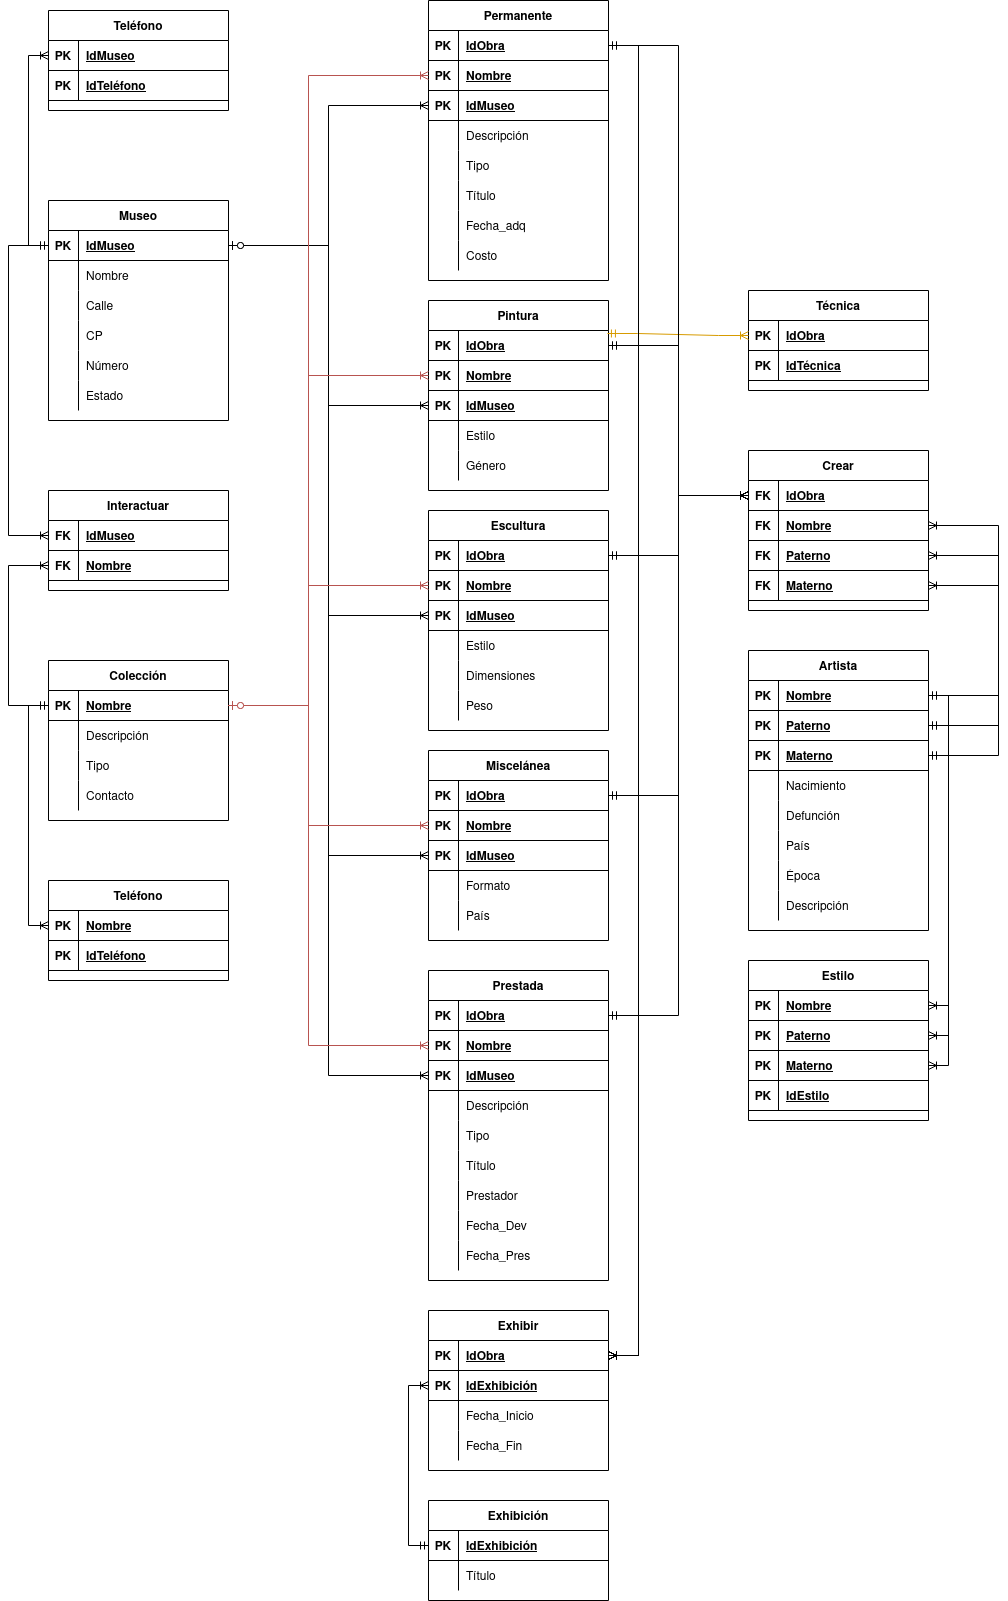
\includegraphics[width=14cm]{../Diagramas/2.png}
    \end{figure}
	
	\newpage
	\question \textbf{Modelo relacional e inserción de tuplas}
	\begin{enumerate}[label=\alph*.]
		\item 
		
	\begin{tabular}{| c | c |}
		\hline
	    Modelo E-R & Modelo Relacional  \\ \hline
        M:N & A(\underline{a1}, \underline{a2}, a3); 
ab(\underline{a1} FK, \underline{a2} FK, \underline{b} FK, ab1); 
B(\underline{b}, b1) \\ \hline
        1:N & A(\underline{a1}, \underline{a2}, a3); 
B(\underline{b}, b1, a1 FK, a2 FK, ab1) \\ \hline
        N:1 & A(\underline{a1}, \underline{a2}, a3, b FK, ab1); 
B(\underline{b}, b1) \\ \hline
        1:1 & A(\underline{a1}, \underline{a2}, a3); 
ab(\underline{a1} FK, \underline{a2} FK, \underline{b} FK, ab1); 
B(\underline{b}, b1) \\ \hline
    \end{tabular} 
	
		\item 
		\begin{enumerate}[label=(\roman*)]
			\item No se inserta completamente, ya que se insertan las cuatro primeras tuplas pero la última duplica la llave primaria (4,'xx',27).
			\item No se inserta ni una tupla, ya que ninguna tiene valores que coincidan con la llave primaria de la relación A.
			\item Si el primer y tercer atributo son a1 y a2 respectivamente, estos forman a la llave primaria de la relación A, de este modo las tuplas de este inciso
sí se pueden insertar completamente.
			\item No se inserta completamente, ya que se insertan las cuatro primeras tuplas pero la última tiene valores para la llave foránea (a1, a2)
que no existen como llave primaria de la relación A.
		\end{enumerate}
		
		\item 
		\begin{enumerate}[label=(\roman*)]
			\item No se inserta ninguna tupla, ya que la llave primaria de la relación A se compone por los primeros dos atributos de esta o el primer y tercer atributo,
por lo que en ninguna de las tuplas del inciso se tienen valores válidos para formar la llave foránea (a1, a2).
			\item Ninguna tupla se puede insertar ya que dado que la relación es de 1:N, donde una tupla de A se asocia con N tuplas de B, la llave foránea (a1, a2) debe
encontrarse en la relación B junto con los atributos de la relación ab del modelo ER. En una relación ningún valor que compone a la llave primaria puede
ser nulo y en las tuplas que se desean insertar sólo se encuentra un atributo de la llave foránea (a1, a2), por lo que faltan los valores para a2 y así
poder hacer referencia a la llave primaria de la relación A.
			\item Los valores para la llave foránea (a1, a2) coinciden con los de la llave primaria de la relación A, los valores de llave primaria de la relación B no se
repiten y si tomamos en cuenta que los valores para b1 son nulos y por ello no se escriben en cada tupla, entonces todas las tuplas se insertan
completamente.
			\item En este caso tampoco se podrá insertar ninguna tupla, ya que aunque la llave primaria de la relación A se formara por el primer y el tercer atributo, ninguno
de los valores para la llave foránea (a1, a2) coincide con los valores de la llave primaria en la relación A.
		\end{enumerate}
			
		\item El modelo relacional quedaría de la siguiente manera:
		
A(\underline{a1}, \underline{a2}, a3, b, ab1)\\
B(\underline{b}, b1)\\

Un conjunto de tuplas que se puede insertar sería:
(2,'ww','a',57,100); (4,'xx','b',17,200); (6,'yy','c',27,300); (8,'zz','d',47,400)
Se pueden insertar ya que ninguna llave primaria se repite (primeros dos atributos) y tampoco se repiten los valores para la llave foránea. Los valores para
a3 y ab1 se encuentran en sus respectivos dominios.

Un conjunto de tuplas que no se podría insertar completamente sería:
(2,'ww','a',57,100); (4,'xx','b',57,200); (4,'xx','c',27,300); (8,42,'d',47,400)
La única tupla que se podría insertar es la primera, la segunda ya no cumple con la relación 1:1 ya que repite el valor para la llave foránea (57), la tercera
trata de duplicar la llave primaria de la segunda, y para a2 en la cuarta no se encuentra el valor en el dominio de las cadenas.
	
		
	\end{enumerate}	
	
	\question \textbf{Modelo relaciones y restricciones de integridad}
	
	\begin{enumerate}[label=(\roman*)]
		\item No, ya que se utiliza el nombre de la compañia (NombreCia) como llave primaria de la relación Compañía, al ser llave primaria no se puede repetir.
		\item Sí es posible, ya que la llave primaria de la relación Dirigir se compone por NombrePersona y NombreCia, por lo que bien pueden existir las tuplas
('Juan', 'Sorny', '2020-01-01', NULL) y ('María', 'Sorny', '2019-05-16', NULL).
		\item Sí puede trabajar en 'Compumundo Hipermegared' y dirigir 'El Bar de Moe' al mismo tiempo, ya que son distintas relaciones y es posible tener una tupla en
cada relación.
		\item Para dirigir 'Leftorium' un empleado no necesariamente debe trabajar en dicha compañía, puede existir una tupla en la relación Trabaja con
'Compumundo Hipermegared' y otra en la relación Dirigir con 'Leftorium', tal como ocurre en el inciso c.
		\item Un empleado no podría dirigir 'Krusty Burgers' en dos períodos de tiempo diferentes, ya que la llave primaria se forma tomando el nombre del empleado y
el nombre de la compañía, por lo que si se desea crear las tuplas ('Juan', 'Krusty Burgers', '2020-01-01', '2020-10-31') y ('Juan', 'Krusty Burgers', '2021-01-01', '2021-10-31')
se estaría duplicando la llave primaria y eso no es permitido.
		\item No, porque la participación es total de lado de Compañía, por lo que es necesario que exista una tupla al menos en la relación Dirigir para 'Laramie Cigarettes'.
		\item No necesariamente, cada empleado puede vivir en una ciudad igual o diferente a donde se encuentra la compañía, no hay una relación que obligue
a que estén en la misma ciudad.
		\item Falso, en la relación Trabaja no está definida una llave primaria, por lo que podrían haber varias tuplas del mismo empleado en la misma
o diferentes compañías y por ende con más de un salario.
		\item Falso, porque aunque el atributo desde puede ser nulo, la participación es total de lado de Trabaja en la relación que tiene con Empleado, por lo que
cada tupla debe hacer referencia a un empleado.
		\item Falso, ya que la relación marca una participación total de lado de Compañía, por lo tanto deberá ser dirigida por al menos un empleado.
		
	\end{enumerate}	
	
	
\end{questions}

\end{document}
